\documentclass[a4paper]{article}
\usepackage[english]{babel}
\usepackage[T1]{fontenc}
\usepackage[utf8x]{inputenc}
\usepackage[a4paper]{geometry}

\geometry{verbose,tmargin=3cm,bmargin=3cm,lmargin=2cm,rmargin=2cm,headheight=2cm,headsep=1cm,footskip=2cm}


\usepackage{enumerate}
\usepackage{enumitem}
\usepackage{adjustbox}
\setlength{\parskip}{\medskipamount}
\setlength{\parindent}{0pt}
\usepackage{graphicx}
\usepackage{listings}
\usepackage{subcaption}
\usepackage{varwidth}
\usepackage{float} 
\usepackage{color}
\usepackage{lastpage}
\usepackage{indentfirst}


% Create header

\usepackage{fancyhdr}
\pagestyle{fancy}
\lhead[lh-even]{Edgar Vedvik\\edgarmv}
\chead[ch-even]{TDT4173 Maskinlæring og case-basert resonnering\\Assignment 2}
\rhead[rh-even]{\today}

\lfoot[lf-even]{}
\cfoot[cf-even]{Page \thepage{} of \pageref{LastPage}}
\rfoot[rf-even]{}


\begin{document}
\newlength{\itemizewidth}% <-- text width in itemize
\setlength{\itemizewidth}{\dimexpr\linewidth-\leftmargini\relax}
\section{Theory}
\begin{enumerate}
    \item
        CBR methods differs from other machine learning approaches in a few
        ways. Other machine learning approaches have a training phase and
        generalizes from the examples given here, in CBR the problem solving is
        lazy, meaning that it waits until a new case is given before doing any
        computation. CBR also stores previous cases or data, whereas other
        machine learning approaches discards the training data as soon as it has
        been used to update their model. 
    \item
        Memory organisation packets (MOPs) is one of the ways cognitive science
        has influenced CBR. MOPs are dynamic memory models, which represents
        classes of situations, their typical goals and the participating actors.
        MOPs are designed to evolve and are interconnected in networks.

        In addition to MOPs, there are thematic organisation packets (TOPs).
        These packets contain general knowledge of the relations between goals
        and event sequences across contexts.
    \item
        \emph{Surface similarity} is concerned with the surface features of the
        cases. These features are provided as part of the case's description and
        is usually represented as attribute-value pairs. The features of the new
        case is compared with experienced cases and given a similarity value,
        which is a number between 0 and 1, where 1 is exactly similar and 0 not
        similar at all. Each of these similarities is weighted based on their
        importance and combined into a global similarity score. An example of
        this can be two patients who both present with the same symptoms, or two
        cases in court where the same crime has been committed.
   
        \emph{Structural similarity} is used when cases are represented by
        complex structures, such as graphs or first-order terms. This type of
        similarity heavily uses domain knowledge. Structural similarity can be
        used to see how similar two buildings are based on the arrangement of the
        rooms, which can be represented as a graph structure. Another example is
        a pipe system which consists of several different parts.
    \item
        Each attribute is compared individually to create a local similarity
        score, then each local similarity score is combined in some way, such as
        giving each attribute a weight, to create the global similarity score.
        This score is used to determine which case is the most similar to this
        one.
    \item
        Case-based reasoning systems store their knowledge in Knowledge
        containers. These containers describe how and where knowledge is stored.
        There are four major knowledge containers: vocabulary, similarity, case
        base and adaptation. These 4 types of knowledge can combined be used to
        solve a problem. 

        \begin{itemize}
            \item
                The vocabulary container determines what can be discussed
                explicitly. For example, the word heart rate must be known in
                order to discuss it. This word and its meaning would be stored
                in the vocabulary container. It is also possible to create
                sub-containers such as names of employees, companies or products
                in a supermarket.
            \item
                The similarity container consists of all knowledge needed to
                determine what makes a case similar to another such that their
                solutions can be reciprocally reused.
            \item
                The case base container contains experiences as cases. The
                experiences may be from the past, constructed from existing
                cases or artificially made.
            \item
                The adaptation container contains knowledge needed to adapt
                cases to solve new problems. Usually this contains rules that
                determine how previous solutions can be transformed to fit a new
                case.
        \end{itemize}
\end{enumerate}
\section{Practical}
\subsubsection*{Case Modelling}
    \begin{enumerate}[label=\alph*)]
        \setcounter{enumi}{2}
        \item
            A screenshot of task a, b and c can be seen in Figure
            \ref{fig:patient}
            \begin{figure}[H]
                \centering
                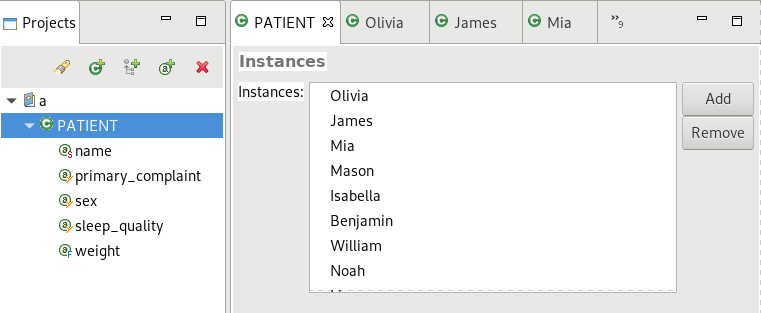
\includegraphics[width=0.7\linewidth]{patient.png}
                \caption{The patient concept with 5 attributes and 12
                instances}
                \label{fig:patient}
            \end{figure}
        \item
            Instances of the patient concept can be seen in Figure
            \ref{fig:instances}

            \begin{figure}[H]
                \centering
                \hfill
                \begin{subfigure}{.47\itemizewidth}%
                    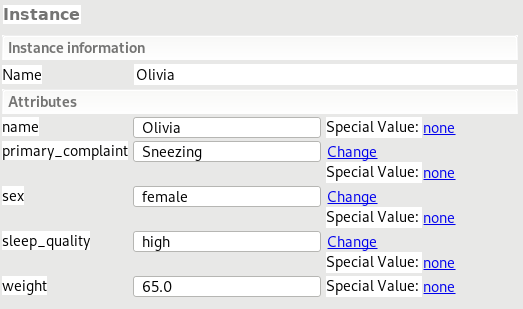
\includegraphics[width=\linewidth]{olivia.png}
                \end{subfigure}
                \hspace{0.05\itemizewidth}
                \begin{subfigure}{.47\itemizewidth}%
                    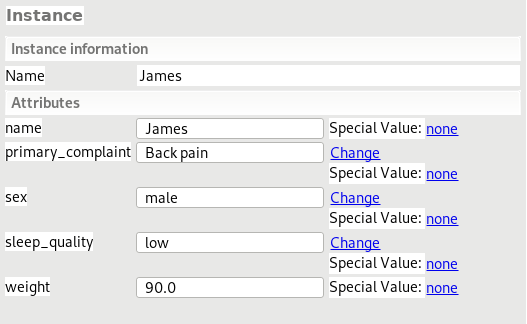
\includegraphics[width=\linewidth]{james.png}
                \end{subfigure}

                \vspace{5mm}

                \begin{subfigure}{.47\itemizewidth}%
                    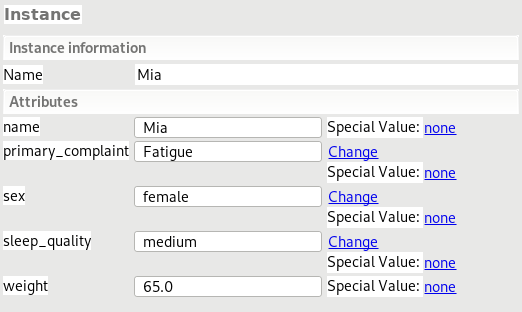
\includegraphics[width=\linewidth]{mia.png}
                \end{subfigure}
                \caption{Three patient instances}
                \label{fig:instances}
            \end{figure}
    \end{enumerate}
\subsubsection*{Case Retrieval}
    \begin{enumerate}[label=\alph*)]
        \setcounter{enumi}{4}
        \item

            Three different similarity measures was created for the weight
            attribute. The first similarity measure gives an exact match a
            similarity score of $1.0$ and then linearly decreases down to $0.0$ the
            further away the weight value is. This similarity measure can be
            seen in Figure \ref{fig:similarity_function}.

            The next measure decreases linearly until the weight value is $±100
            kg$ away, here it is given a similarity score of $0.1$. Then decreases
            linearly from this point as well.

            The third measure is a smooth step function at $±30 kg$. This means
            that weight values closer than $30 kg$ is given a near $1.0$ score (with
            exact match a full $1.0$ score), and weight values further than $30 kg$
            apart a close to $0.0$ similarity score.

            \begin{figure}[H]
                \centering
                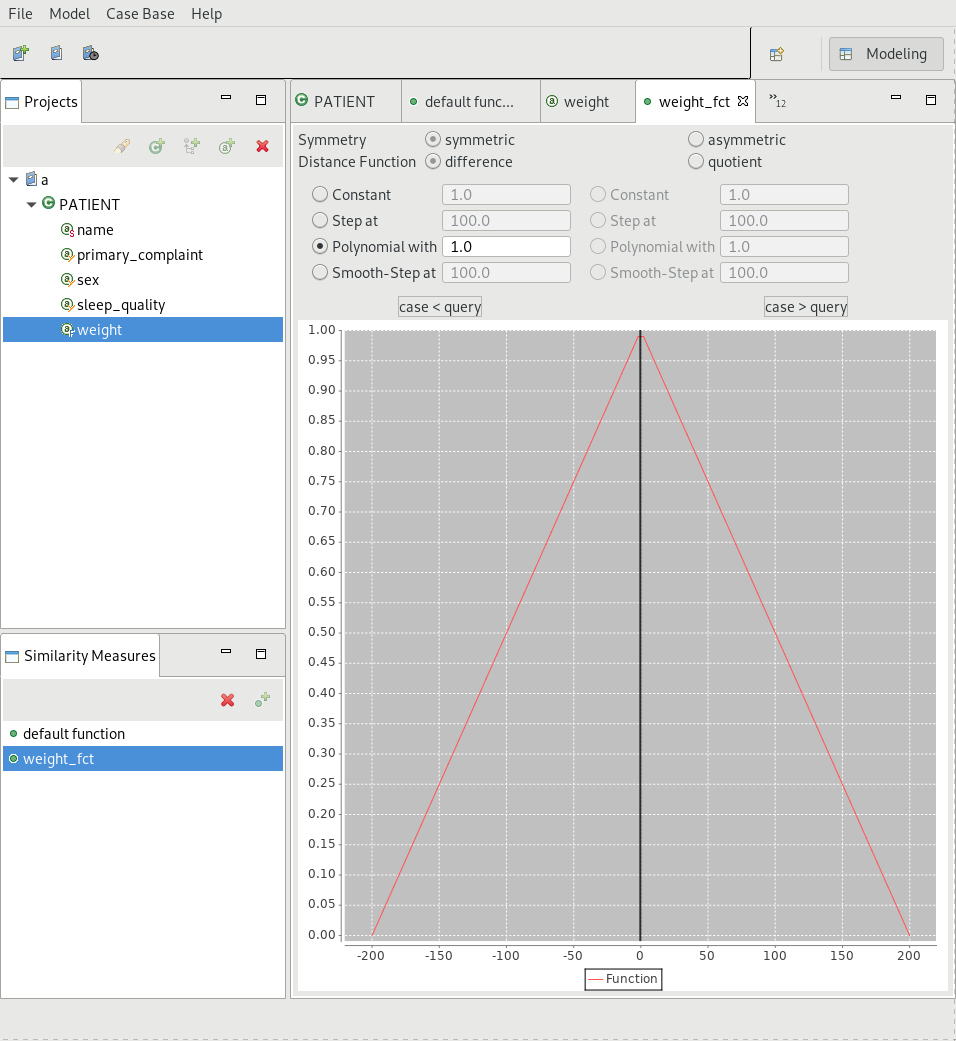
\includegraphics[width=0.7\linewidth]{similarity_function.png}
                \caption{A similarity measure for the weight attribute}
                \label{fig:similarity_function}
            \end{figure}

            The global similarity measure is shown in Figure
            \ref{fig:global_sim}. Here the name and sex attributes are ignored.
            The weight attribute uses the smooth step function explained
            previously. The sleep quality function makes high and medium
            similar, medium and low similar, but high and low is not very
            similar. Finally, the primary\_complaint similarity measure makes
            symptoms that (I think) are similar score high, such as back pain
            and joint pain. Symptoms that I consider not similar is given a low
            score, such as back pain sneezing.

            \begin{figure}[H]
                \centering
                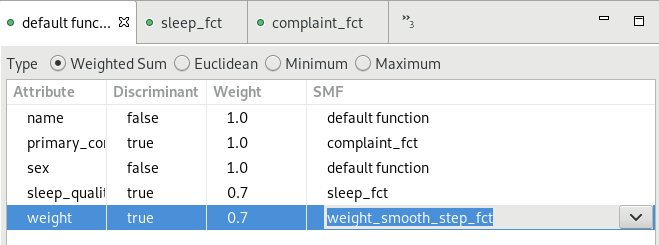
\includegraphics[width=0.7\linewidth]{global_function.png}
                \caption{The global similarity measure for the patient concept.}
                \label{fig:global_sim}
            \end{figure}
        \item
            In Figure \ref{fig:retrieval1} a retrieval query for a complaint of
            stomach problems, high sleep quality and a weight of $100kg$ was issued.
            The top three results for this were Benjamin, Liam, and Isabella, with
            similarity scores 0.88, 0.58 and 0.48 respectively. Benjamin, the
            highest scorer, had a complaint of stomach problems, medium sleep
            quality and weighed $90kg$. This scored high because the complaints
            were similar, and the sleep quality differed little. The weights
            were also similar.

            The next result, Liam, only scored 0.58. His case has primary
            complaint as join pain, sleep quality as high and weighs $95kg$.
            This result shows how much the primary complaint affects the
            similarity scores. Since stomach problems and joint pain does not
            have much in common he scores poorly, even though his sleep quality
            and weight matches better than Benjamin.

            The third result, Isabella, is 0.48 similar. Isabella's case
            consists of a stomach problem complaint, low sleep quality and a
            weight of $60$kg. The reason for such a low score is because
            Isabella is outside the $30kg$ difference in our weight function,
            which means her weight score is 0. Her sleep quality is also far
            from the queried sleep quality, and therefore having the same
            complaint is the only thing that is similar in these two cases.

            
            \begin{figure}[H]
                \centering
                \hfill
                \begin{subfigure}{.47\itemizewidth}%
                    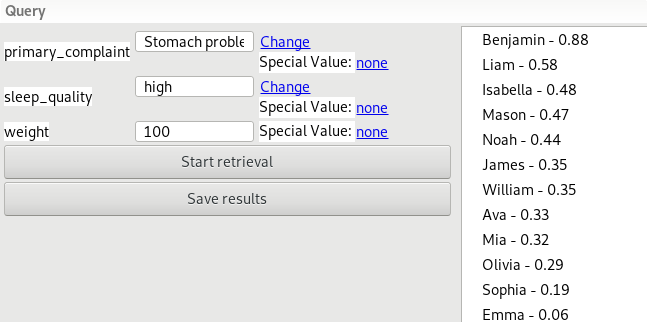
\includegraphics[width=\linewidth]{retrieval1.png}
                    \caption{}
                    \label{fig:retrieval1}
                \end{subfigure}
                \hspace{0.05\itemizewidth}
                \begin{subfigure}{.47\itemizewidth}%
                    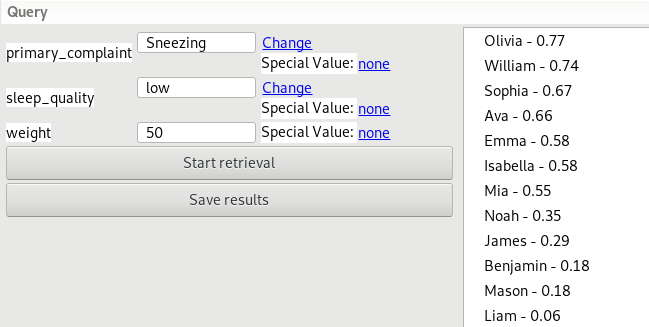
\includegraphics[width=\linewidth]{retrieval2.png}
                    \caption{}
                \end{subfigure}

                \vspace{5mm}

                \hfill
                \begin{subfigure}{.47\itemizewidth}%
                    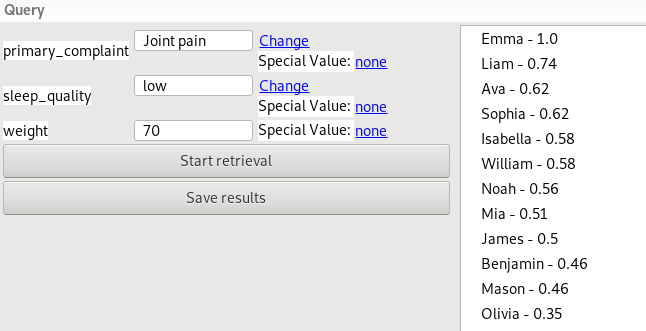
\includegraphics[width=\linewidth]{retrieval3.png}
                    \caption{}
                \end{subfigure}
                \hspace{0.05\itemizewidth}
                \begin{subfigure}{.47\itemizewidth}%
                    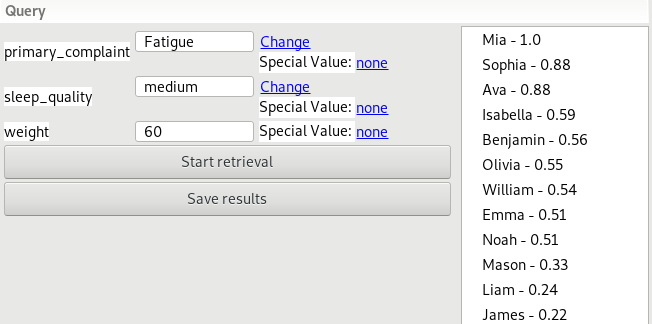
\includegraphics[width=\linewidth]{retrieval4.png}
                    \caption{}
                \end{subfigure}

                \vspace{5mm}

                \begin{subfigure}{.47\itemizewidth}%
                    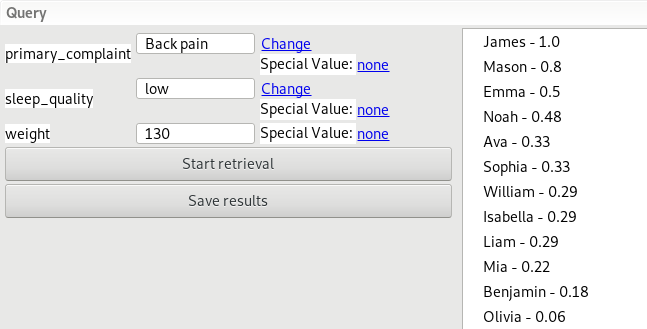
\includegraphics[width=\linewidth]{retrieval5.png}
                    \caption{}
                    \label{fig:retrieval5}
                \end{subfigure}
                \caption{Five retrieval queries.}
            \end{figure}

            None of the results are unexpected, Some of the queries resulted in
            a 1.0 match when the complaint and sleep quality matched and the
            weight was within a $±30$ range. Other results scored close to zero
            (0.06 for Olivia in Figure \ref{fig:retrieval5}). This is caused by
            a large gap in their weights, symptoms that are not similar and
            different sleep quality.
            
        \item
            Diagnosing patients is a common problem for doctors, and since the
            primary complaint attribute already existed this is the problem I
            have decided to use for the patient concept. In order to do this I
            added a diagnosis attribute with type string. Then I gave all
            instances of patient a diagnosis fitting with their complaint. In
            the global similarity measure I disabled the diagnosis attribute
            since it should not be used to determine similarity.

            The four steps in the CBR-cycle can be executed in myCBR as follows:

            \begin{itemize}
                \item
                    \textbf{Retrieve} is done by executing a retrieval in myCBR with
                    the new problem as query parameters. This gives a list of
                    the most similar cases.
                \item
                    \textbf{Reuse} can be done simply by looking under the top
                    result to see what diagnosis the retrieved patient was
                    given. This diagnosis can then be used for the new patient.
                \item
                    \textbf{Revision} is done manually, after finding a solution,
                    the user of myCBR can revise the solution if necessary.
                \item
                    \textbf{Retain} is done by adding a new instance to the case
                    base with the query parameters and the solution from the
                    retrieve or revise steps.
            \end{itemize}

    \end{enumerate}
\end{document}
